%% Version 4.3.2, 25 August 2014
%
%%%%%%%%%%%%%%%%%%%%%%%%%%%%%%%%%%%%%%%%%%%%%%%%%%%%%%%%%%%%%%%%%%%%%%
% Template.tex --  LaTeX-based template for submissions to the 
% American Meteorological Society
%
% Template developed by Amy Hendrickson, 2013, TeXnology Inc., 
% amyh@texnology.com, http://www.texnology.com
% following earlier work by Brian Papa, American Meteorological Society
%
% Email questions to latex@ametsoc.org.
%
%%%%%%%%%%%%%%%%%%%%%%%%%%%%%%%%%%%%%%%%%%%%%%%%%%%%%%%%%%%%%%%%%%%%%
% PREAMBLE
%%%%%%%%%%%%%%%%%%%%%%%%%%%%%%%%%%%%%%%%%%%%%%%%%%%%%%%%%%%%%%%%%%%%%

%% Start with one of the following:
% DOUBLE-SPACED VERSION FOR SUBMISSION TO THE AMS
\documentclass{ametsoc}

% TWO-COLUMN JOURNAL PAGE LAYOUT---FOR AUTHOR USE ONLY
% \documentclass[twocol]{ametsoc}

%%%%%%%%%%%%%%%%%%%%%%%%%%%%%%%%
%%% To be entered only if twocol option is used

\journal{jamc}

%  Please choose a journal abbreviation to use above from the following list:
% 
%   jamc     (Journal of Applied Meteorology and Climatology)
%   jtech     (Journal of Atmospheric and Oceanic Technology)
%   jhm      (Journal of Hydrometeorology)
%   jpo     (Journal of Physical Oceanography)
%   jas      (Journal of Atmospheric Sciences)	
%   jcli      (Journal of Climate)
%   mwr      (Monthly Weather Review)
%   wcas      (Weather, Climate, and Society)
%   waf       (Weather and Forecasting)
%   bams (Bulletin of the American Meteorological Society)
%   ei    (Earth Interactions)

%%%%%%%%%%%%%%%%%%%%%%%%%%%%%%%%
%Citations should be of the form ``author year''  not ``author, year''
\bibpunct{(}{)}{;}{a}{}{,}

%%%%%%%%%%%%%%%%%%%%%%%%%%%%%%%%

%%% To be entered by author:

%% May use \\ to break lines in title:

\title{Verifying Operational Forecasts of Land-Sea Breeze and Boundary Layer Mixing Processes}

%%% Enter authors' names, as you see in this example:
%%% Use \correspondingauthor{} and \thanks{Current Affiliation:...}
%%% immediately following the appropriate author.
%%%
%%% Note that the \correspondingauthor{} command is NECESSARY.
%%% The \thanks{} commands are OPTIONAL.

    %\authors{Author One\correspondingauthor{Author One, 
    % American Meteorological Society, 
    % 45 Beacon St., Boston, MA 02108.}
% and Author Two\thanks{Current affiliation: American Meteorological Society, 
    % 45 Beacon St., Boston, MA 02108.}}

\authors{Ewan Short\correspondingauthor{School of Earth Sciences, The University of Melbourne, Melbourne, Victoria, Australia.}} 

\email{shorte1@student.unimelb.edu.au}

%% Follow this form:
    % \affiliation{American Meteorological Society, 
    % Boston, Massachusetts.}

\affiliation{School of Earth Sciences, and ARC Centre of Excellence for Climate Extremes, The University of Melbourne, Melbourne, Victoria, Australia.}

%% Follow this form:
    %\email{latex@ametsoc.org}

%\email{}

%% If appropriate, add additional authors, different affiliations:
    %\extraauthor{Extra Author}
    %\extraaffil{Affiliation, City, State/Province, Country}

\extraauthor{Ben \textcolor{red}{?}. Price}

\extraaffil{Bureau of Meteorology, Casuarina, Northern Territory, Australia}

\extraauthor{Derryn \textcolor{red}{?}. Griffiths and Alexei \textcolor{red}{?}. Hider}

\extraaffil{Bureau of Meteorology, Melbourne, Victoria, Australia}

\DeclareMathOperator{\mse}{mse} 
\DeclareMathOperator{\covar}{covar} 
\DeclareMathOperator{\var}{var} 
\DeclareMathOperator{\pr}{Pr} 

%\extraauthor{}
%\extraaffil{}

%% May repeat for a additional authors/affiliations:

%\extraauthor{}
%\extraaffil{}

%%%%%%%%%%%%%%%%%%%%%%%%%%%%%%%%%%%%%%%%%%%%%%%%%%%%%%%%%%%%%%%%%%%%%
% ABSTRACT
%
% Enter your abstract here
% Abstracts should not exceed 250 words in length!
%
% For BAMS authors only: If your article requires a Capsule Summary, please place the capsule text at the end of your abstract
% and identify it as the capsule. Example: This is the end of the abstract. (Capsule Summary) This is the capsule summary. 

% Run "latexdiff --append-context2cmd="abstract" short18_diurnal_cycles_winds.tex short18_diurnal_cycles_winds_revised.tex > short18_diurnal_cycles_winds_tracked_changes.tex" to track changes

\abstract{This study presents a method for verifying the diurnally varying component of operational wind forecasts that are typically based on model data that is then edited by human forecasters. The model datasets most commonly used by Australian forecasters for winds are those of the European Center for Medium-Range Weather Forecasting (ECMWF) and the Australian Community Climate and Earth System Simulator (ACCESS). The methodology is applied to the coastal weather stations across Australia over June, July and August 2018, at three different spatial scales, on both a daily and seasonal basis. The results indicate that while the Official forecast outperforms unedited ACCESS and ECMWF at certain locations and times of day, it rarely outperforms both at once. The causes of the differences in the performance of each dataset vary by location, but can include biases in the direction at which the sea-breeze approaches the coast, amplitude biases in the diurnal cycle, and disagreement as the whether sea-breeze or boundary layer mixing processes contribute most to the diurnal cycle. Furthermore, when winds are compared at small spatial scales on a daily basis, ECMWF outperforms Official and ACCESS simply because its coarser resolution creates less internal variability than Official or ACCESS. These results have implications for both forecasting practice and verification methodology.}

\usepackage{comment}

\begin{document}

\maketitle

\section{Introduction}
\label{Sec:Introduction}
Modern weather forecasts are typically produced by models in conjunction with human forecasters. Forecasters working for the Australian Bureau of Meteorology (BoM) construct a seven day forecast by loading model data into a software package called the Graphical Forecast Editor (GFE), then editing this model data using tools within GFE. \textcolor{red}{Is this also how things work at the U.S~National Weather Service and U.K.~Met Office?} Forecasters can choose which model to base their forecast on, and refer to this as a choice of \textit{model guidance}. Edits are typically made to account for processes that are under-resolved at synoptic scale model resolutions, or to correct known biases of the models being used. The resulting gridded forecast datasets are then provided to the public through the BoM's online MetEye data browser \citep{bomMetEye19}; the gridded forecast datasets are also translated into text and icon forecasts algorithmically.  

Australian forecasters generally make two types of edits to the surface wind fields on a routine daily basis. The first is to edit the surface winds after sunrise at locations where the forecaster believes the model guidance is providing a poor representation of boundary layer mixing processes. Bounday layer mixing occurs as the land surface heats up, producing an unstable boundary layer which transports momentum downward to the surface layer, where winds are both weaker and ageostrophically oriented due to surface friction \citep{lee18}. The forecaster may edit both speed and direction on the basis of climatological knowledge, theory or recent upper level wind soundings from nearby stations. \textcolor{red}{How do the boundary layer mixing tools in GFE currently work? While I was in Darwin you picked a height $z$ and a percentage $p$, and the tool essentially formed an average of the surface winds and winds at $x$ weighted by $p$.}

The second type of edit involves changing the afternoon and evening surface winds around those coastlines where the forecaster believes the model guidance is resolving the sea-breeze poorly. \textcolor{red}{How do the sea-breeze tools in GFE currently work? While I was in Darwin you traced out the relevant coastline graphically, chose a wind speed and a time, and GFE would add in winds perpendicular to the traced coastline at this speed, and smoothly blend them in spatially and temporally.} 

\begin{table}
\begin{center}
\begin{tabular}{l |c|c}
Airport & Austral Summer & Austral Winter \\
\hline
Darwin  & 6.3 kn& 6.2 kn \\
Brisbane  & 8.6 kn& 7.0 kn \\
Perth  & 11.3 kn& 7.9 kn \\
Sydney  & 12.2 kn & 10.2 kn \\
Adelaide  & 9.5 kn & 10.3 kn \\
Canberra  & 7.4 kn & 7.9 kn \\
Melbourne  & 10.0 kn & 12.1 kn \\
Hobart & 10.0 kn & 8.7 kn
\end{tabular}
\caption{Average 10 m wind speeds for austral winter (June, July August) 2018, and austral summer (December, January, February) 2017/18 across the eight Australian capital city airport weather stations.}
\label{Tab:Speeds}
\end{center}
\end{table}

Forecasters and national weather services have good reasons for ensuring the diurnally varying component of their wind forecasts are as accurate as possible. \citet{dai99} fitted the first two harmonics to seasonal averages of wind speed at different times of day and showed that over land surfaces the average amplitude of the wind speed diurnal cycle varied from $1.2$ to $2.1$ kn, \textcolor{red}{(knots are used throughout this paper because this is the unit forecasters work with, and the unit that is used in Jive)} and that the fitted harmonics accounted for $50$ to $70\%$ of the daily variability. Table \ref{Tab:Speeds} shows the mean wind speeds for the Australian capital city airport station shown in Fig.~\ref{Fig:map}, over December, January, February 2017/18 and June, July and August 2018, suggesting that the amplitude of the mean diurnal cycles are approximately $10$ to $34\%$ of the mean wind speeds across Australia. 

Beyond their contribution to the overall wind field, diurnal wind cycles are important in and of themselves to the ventilation of pollution, with sea-breezes transporting clean maritime air inland, where it helps flush polluted air out of the boundary layer \citep{miller03}. The Victorian Latrobe Valley provides an important Austrailan example of this effect \citep{physick92}. Furthermore, diurnal wind cycles affect the function of wind turbines \citep{englberger18} and the design of wind farms \citep{abkar16}, as daily patterns of boundary layer stability affect turbine wake turbulence, and the losses in wind power that result. 

To our knowledge, no published work has assessed the diurnal component of human edited forecasts, although some previous studies have assessed the performance of different operational models at specific locations. \citet{svensson11} examined thirty different operational model simulations, including models from most major forecasting centres utilising most commonly used boundary layer parametrisation schemes, and compared their performance with a large eddy simulation (LES), and observations at Kansas, USA during October 1999. They found that both the models and LES failed to capture the sudden $\approx 6$ kn jump in wind speeds shortly after sunrise, and underestimated morning low level turbulence and wind speeds. Other studies have assessed near-surface wind forecasts, verifying the total wind speeds, not just the diurnal component. \citet{pinson12} performed a verification study of the 10 m wind speeds resolved by the European Centre for Medium Range Weather Forecasting (ECMWF) operational model ensemble across western Europe over December, January, February 2008/09. They found that the worst performing regions were coastal and mountainous areas, and attributed this poor performance to the small scale processes, e.g. sea and mountain breezes, that are under-resolved at ECMWF's coarse 50km spatial resolution. 

Any attempt to validate model data against observations must confront the \textit{representation problem} \citep[e.g.][]{zaron06}. Because models cannot resolve physical processes occurring at sub-grid scales, a value predicted by an operational model for a given grid-cell must be interpreted as a prediction of the filtered, or Reynolds averaged value over that grid-cell. While strictly speaking, observational instruments also impose a degree of filtering on reality, in the case of the AWS observations considered here, the filtering is much less than for the model predictions. Therefore, comparing model data with observational data can be an unfair test of model performance, and for this reason model forecasts are often verified against reanalysis hind-casts that use the same model \citep[e.g.][]{lynch14}.

However, the way the representation problem applies to the verification of forecasts issued to the public is more nuanced. In this case, a forecast issued by a national weather service is attempting to represent either reality itself, or the filtered version of reality \textit{that is of interest to the end user.} Thus, \citet{pinson12} disregarded the representation problem entirely, arguing that the end user is not interested in spatiotemporal scales of models, only the best representation of reality at the time and place of their choice. However, it is hard \textcolor{red}{(impossible)} to completely escape making assumptions about the filtered version of reality the end user wants from a forecast. BoM wind verification scores used internally are derived by comparing hourly Official forecast data with station observations that are averaged 10 minutes either side of the hour: implicit in this practice is the assumption that the user does not care about wind turbulence at temporal scales less than 20 minutes. Beyond this, the fact that the Official forecast is formed from model datasets with different resolutions, with the choice of model guidance changing over the course of a single day, e.g.~Fig.~\ref{Fig:case_studies} c), makes the precise version of reality the Official forecast is intending to represent unclear, and hence addressing the representation problem difficult. \textcolor{red}{The point I'm trying to make here is perhaps unclear. Essentially I'm arguing that the representation problem applies, but although the intended filtered version of reality represented by a particular model is clear, it is not clear in the Official forecast due to it's hybrid structure, and because what it intends to represent is perhaps not clear to the user, or consistent between different users. Note that clicking locations on the MetEye map seems to bring up the forecast for the nearest station or population centre. Does this imply that the Official forecast is intending to represent spatial scales at least as fine as the distance between stations? Or is it intending to represent averaged parameters at the ACCESS-R or ACCESS-C resolutions? Note also that grids are only provided every 3 hours in MetEye; do these grids represent the hourly values from the Official forecast, provided just at these three hour intervals, or a three hourly average?}

Related to the representation problem is the question of how mesoscale models, which run at spatial resolutions of between 1 and 10 km, should be verified. This question is of relevance to the present study as the BoM now regularly runs mesoscale models over some Australian capital cities as part of its daily forecasting routine, and the edits performed by human forecasters are also often performed at the mesoscale. Mesoscale models resolve topography and its effects on the atmosphere in more detail, and explicitly simulate most convective and boundary layer processes. In this sense they are more realistic than coarser scale synoptic models, although they can actually perform worse than coarse models on standard verification scores whenever there are timing or location differences between features in the models and in observations. \citet{mass02} found that in the northwestern United States, mean square error scores in forecasts produced using a mesoscale model decreased with resolution down to 10 to 15 km, whereas in the eastern United States where the topography is much flatter, this threshold was considerably larger, at 20 to 40 km. 

\citet{mass02} therefore argued that existing verification approaches needed reform, suggesting that verification could instead be performed on spatially or temporally averaged parameters, an approach now known as \textit{upscaling} \citep{ebert08}, or that ``feature based" identification metrics be developed, which reward models for realistically simulating atmospheric features, even if the timing or location of these features is slightly incorrect. \citet{ebert00} developed such a method for precipitation, focusing on spatial displacements and differences in the shapes of the rainfall areas between observations and models. \citet{rife05} applied similar ideas to the verification of surface winds, defining a wind ``object" as a wind change of at least one standard deviation occurring within a 12 hour interval, then assessing whether a mesoscale model could replicate the ``objects" present in observations.   

The present study has two goals. First, to describe a method for comparing the diurnal cycles of human edited wind forecasts to those of unedited model guidance forecasts, in order to assess where and when human edits produce an increase in accuracy, and to do so in a way that respects the representation and mesoscale verification challenges discussed above. Second, to apply this methodology across Australian coastal locations to better understand the performance of both boundary layer mixing and land-sea breeze forecaster edits. The remainder of this paper is organised as follows. Section \ref{Sec:Methods} describes the methodology and datasets to which it is applied, section \ref{Sec:Results} provides results, and sections \ref{Sec:Discussion} and \ref{Sec:Conclusion} provide a discussion and a conclusion, respectively.

\section{Data and Methods} \label{Sec:Methods}
This study compares both human edited and non human edited Australian Bureau of Meteorology wind forecasts with automatic weather station (AWS) data across Australia. The comparison is performed by first isolating the diurnal signals of each dataset, then comparing these signals on an hour-by-hour basis. Much of the analysis is conducted through the BoM's \textit{Jive} verification platform \textcolor{red}{(Provide either a URL link to an Official Jive page if one exists by the time of publication, or a link to copy of Jive I've been using on my laptop, which I could host on my personal GitHub page.)}, which provides an archive of forecast, model guidance and observational data, and a software library for calculating basic statistics.  

\subsection{Data} 
Four datasets are considered in this study; the Official BoM wind forecast data that is issued to the public, model data from ECMWF, \textcolor{red}{(is this the mean of the ECMWF operational ensemble?)} model data from the Australian Community Climate and Earth System Simulator (ACCESS), \textcolor{red}{(I haven't considered the BoM's Operational Consensus Forecast in this study, because it was not used in the Official forecast for winds while I was in the NT. If it is used in other states, the study can be reinterpreted as a verification of both forecaster edits and OCF against unedited, un-post-processed model guidance.)} and observational data from automatic weather stations (AWS) across Australia. \textcolor{red}{(With the Bureau's permission, I would like to make the datasets used in this paper open access, and host them on the NCI catalogue page.)} The Official and ECMWF data are at a \textcolor{red}{?, ?} degree spatial resolution respectively. \textcolor{red}{What are the resolutions of these datasets as they're used in Jive? I know ACCESS uses nested grids, so what is the resolution of the ACCESS dataset when used in GFE and Jive? Are the outer grids interpolated to the resolution of the inner grids, or are the inner grids upscaled?} Official, ACCESS and AWS data exists at each UTC hour, but ECMWF data only exists at a three hour resolution. \textcolor{red}{Why is this? What are the actual time-steps of the models?} To be consistent with the other data sets, ECMWF is therefore linearly interpolated to an hourly resolution: note that this is also what happens when forecasters load ECMWF wind data into the GFE, and the linearly-interpolated ECMWF data is therefore an appropriate model guidance dataset to compare with Official. To facilitate comparison with observations, Official, ACCESS and ECMWF data is \textcolor{red}{(tri-linearly?)} interpolated in all three spatial dimensions to the locations of the weather stations. AWS wind data is recorded every minute at each station, and the hourly AWS datasets used in Jive for this study, and all other internal BoM wind verification studies, are formed by averaging 10 minutes either side of each UTC hour. \textcolor{red}{(My memory is that Jive uses a ten minute average either side, but need to confirm this as it could be five minutes either side.)}

Both ACCESS and ECMWF use parametrisation schemes to simulate sub-grid scale boundary layer turbulence, and the resultant mixing. ACCESS uses the schemes of \citet{lock00} and \citet{louis79} for unstable and stable boundary layers respectively \citep{bom10}. ECMWF uses similar schemes that they develop in-house \citep{ecmwf18}. Data covers the austral winter months of June, July and August 2018; this short time period was chosen to reduce the effect of changing seasonal and climatic conditions, changing forecasting practice and staff, and of developments to the ACCESS and ECMWF models.

\begin{figure*}
\centering
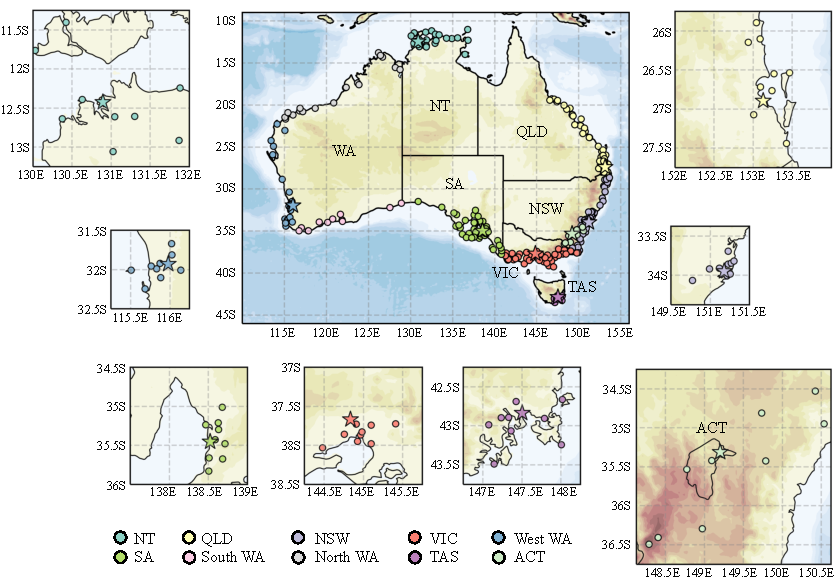
\includegraphics[width=39pc]{map.pdf}
\caption{Locations of the automatic weather stations used in this study. Stars indicate capital city airport stations. Height and depth shading intervals every 200 and 1000 m, respectively.}
\label{Fig:map}
\end{figure*}

\subsection{Assessing Diurnal Cycles}
The overall surface diurnal wind signal includes land-sea breezes, boundary layer mixing processes, mountain-valley breezes, atmospheric tides, and urban heat island circulations. Forecasters typically edit model output to account for under-resolved sea-breezes and boundary layer mixing processes. Instead of attempting to assess each type of edit individually, we study the overall diurnal signal by subtracting a twenty hour centred running mean \textit{background wind} from each zonal and meridional hourly wind data point. This provides a collection of zonal and meridional wind \emph{perturbation} datasets. 

One measure of the accuracy of the Official, ACCESS and ECMWF diurnal cycles is to compare the Euclidean distances of the perturbations at each hour with the corresponding AWS perturbations. For example, to assess whether the Official forecast perturbations, $\boldsymbol{u}_{\text{O}}$, or ACCESS perturbations, $\boldsymbol{u}_{\text{A}}$, best match the AWS observations, $\boldsymbol{u}_{\text{AWS}}$, we calculate the \textit{Wind Perturbation Index} (WPI), defined by 
\begin{equation}
\text{WPI}_\text{OA} = \left\lvert \boldsymbol{u}_{\text{AWS}}-\boldsymbol{u}_{\text{A}} \right\rvert - \left\lvert \boldsymbol{u}_{\text{AWS}}-\boldsymbol{u}_{\text{O}} \right\rvert. \label{Eq:WPI}
\end{equation} 
The analogously defined quantities $\text{WPI}_\text{OE}$ and $\text{WPI}_\text{EA}$ can then be used to provide a comparison of the Official and ECMWF perturbations, and of the ACCESS and ECMWF perturbations, respectively. We can then take means of the WPI on an hourly basis; i.e.~all the 00:00 UTC WPI values are averaged, all the 01:00 UTC values are averaged, and so forth, and denote such an average by $\overline{\text{WPI}}$. 

$\overline{\text{WPI}}$ is the difference of two mean absolute errors. A $\overline{\text{WPI}}_\text{OA}$ value of $0.5$ kn at 00:00 UTC means that the Official 00:00 UTC perturbations are, on average, $0.5$ kn closer to the observed perturbations than are those of ACCESS. The $\text{WPI}$ compares just \textit{one aspect} of the Official forecast with model guidance; it says nothing, for instance, about whether the variability of the Official forecast is closer to that of the AWS than the model guidance. As such, any statements about performance made throughout this paper refer solely to WPI, and no claim is being made that WPI is sufficient to completely characterise the accuracy, or value to the user, of how the surface diurnal wind cycle is represented in competing forecasts.

Note that sea-breeze and boundary layer mixing processes depend crucially on the background atmospheric conditions in which they occur. By comparing wind perturbations rather than the overall wind fields we are not claiming these background conditions are irrelevant. However, when a forecaster makes an edit of a wind forecast to better resolve these processes, they are implicitly assuming that future background conditions will be close enough to either climatology, or model predictions of background conditions themselves, to justify making the edit. Thus, it makes perfect sense to compare forecast perturbations to observed perturbations, as long as errors are interpreted as the consequence not only of how the forecaster or model resolves the diurnal cycle, but of how errors in the background state contribute to errors in the perturbations. To minimise the significance of background state errors, this study focuses exclusively on lead-day one forecasts.

Given the large degree of turbulence and unpredictable variability in both the AWS, Official, and model datasets, care must be taken to ensure we do not pre-emptively conclude Official has outperformed the model guidance when $\overline{\text{WPI}}>0$ purely by chance. The method for estimating confidence in $\overline{\text{WPI}}$ is based on a method proposed by \citet{griffiths17} as a general framework for BoM verification metrics. Note first that WPI is defined so as to minimise the temporal autocorrelations within each dataset, and to avoid having to consider correlations between the zonal and meridional components within and between datasets. Time series formed from the WPI values at a particular time, say 00:00 UTC, across the three month time period, can therefore be idealised as an independent random sample of a random variable $W$. The sampling distribution for each $\overline{\text{WPI}}$ can be modelled by a Student's $t$-distribution, and from this we calculate the probability that $W$ is positive, denoted $\pr\left(W > 0\right)$. Although temporal autocorrelations of WPI, i.e.~correlations between WPI values at a particular hour from one day to the next, are in practice small or non-existent thanks to how WPI is defined, they are still accounted for by reducing the ``effective" sample size to $ n \left(1-\rho_1\right)/\left(1+\rho_1\right)$, where $n$ is the actual sample size and $\rho_1$ is the lag-1 autocorrelation \citep{zwiers95,wilks11}. Note that in the standard language of statistical hypothesis testing, we would reject the null hypothesis that $W=0$ at significance level $\alpha$ if $\pr(W>0) > 1-\frac{\alpha}{2}$ or $\pr(W<0) > 1-\frac{\alpha}{2}$. However, in this study we are interested in both whether $W>0$ or whether $W<0$, so prefer to simply state the value of $\pr(W>0)$, referring to this as a \textit{confidence score}, and noting $\pr(W<0) = 1- \pr(W>0)$. We say Official outperforms model guidance with ``high confidence" if $\pr(W>0) \geq 95\%$, or that model guidance outperforms Official with ``high confidence" if $\pr(W>0) \leq 5\%$, with high confidence implicit whenever it is not explicitly mentioned. \textcolor{red}{Much of this explanation is probably unnecessary, but would like to get feedback before I trim it.}

To investigate the consequences of the representation and mesoscale verification challenges discussed in section \ref{Sec:Introduction}, we apply \textit{upscaling} \citep{ebert08}, where forecast and observational data are first averaged to coarser spatiotemporal scales before being compared. In this study we consider three spatial and two temporal scales. The finest spatial scale is that of the individual station. This study focuses on the 8 capital city airport stations, marked by stars in Fig.~\ref{Fig:map}, as their high operational significance means that they are typically the most accurate and well maintained. The next spatial scale is formed by taking the 10 stations closest to each capital city airport station, with some flexibility allowed to ensure stations are roughly parallel to the nearest coastline. These station groups are referred to as the \textit{airport station groups}. The coarsest spatial scale is formed by taking all stations within 150 km of the nearest coastline, and grouping these by state. This is done because Australian forecasts are currently produced on a state by state basis at forecasting centres based in each state capital, with each forecasting centre utilising different staff, different model guidance preferences, and different editing practices. Indeed, the Official gridded forecast typically shows slight discontinuities across state boundaries \citep{bomMetEye19}. Note that the Western Australian coastline is subdivided into three pieces, and stations along the Gulf of Carpentaria, north Queensland Peninsula, and Tasmanian coastlines are neglected, in order to ensure each station group corresponds to an approximately linear segment of coastline, so as to best resolve the land-sea breeze signal after spatial averaging \citep[e.g.][]{vincent16}. These eight station groups are referred to as the \textit{coastal station groups}.

We also consider both daily and seasonal time scales. For daily time scales, we either consider just the individual airport stations, or modify the definition of WPI in equation (\ref{Eq:WPI}) so that each perturbation dataset is first spatially averaged over either the airport or coastal station groups. Confidence scores are calculated for the airport and coastal station groups in the same way as for the single airport stations, treating the spatially averaged data as a single time series. This provides a conservative way to deal with spatial correlation between the stations in each group \citep{griffiths17}. 

For the seasonal scale comparison we define the \textit{Climatological Wind Perturbation Index} (CWPI) by
\begin{equation}
\text{CWPI}_{\text{OA}} = \left\lvert \overline{\boldsymbol{u}}_{\text{AWS}}-\overline{\boldsymbol{u}}_{\text{O}} \right\rvert - \left\lvert \overline{\boldsymbol{u}}_{\text{AWS}}-\overline{\boldsymbol{u}}_{\text{A}} \right\rvert,
\end{equation}
where the over-bars denote temporal averages of the perturbations at a particular hour, across the three month time period. These temporally averaged perturbations represent the climatological diurnal wind cycle over the three month study period for each dataset. As with the WPI, $\text{CWPI}_{\text{OE}}$ and $\text{CWPI}_{\text{EA}}$ are defined analogously. The three spatial scales are considered in the same way as for WPI, with the spatial average taken before the temporal average. Note that the upscaling method provides another motivation for considering perturbations rather than the overall wind fields, as this prevents the averaged diurnal cycles being washed out by larger scale variability. Uncertainty in the CWPI is estimated through bootstrapping \citep{efron79}. This is done by performing resampling with replacement on the underlying perturbation datasets, and calculating the CWPI multiple times using these resampled datasets. This provides a distribution of CWPI values, which analogously to with WPI, we treat as a sample from a random variable $C$, and use this to estimate $\pr\left(C > 0\right)$.

Although the WPI and CWPI provide quantitive information on the accuracy of the diurnal cycle at different times of day, they do not provide much information on the structure of the diurnal wind cycles of each dataset. \citet{gille05} obtained summary statistics on the observed structure of the climatological diurnal wind cycles across the globe by using linear regression to calculate the coefficients $u_i$, $v_i$ $i=0,1,2$, for the fits 
\begin{align}
u &= u_0 + u_1 \cos(\omega t) + u_2 \sin(\omega t), \label{Eq:u_h} \\
v &= v_0 + v_1 \sin(\omega t) + v_2 \sin(\omega t), \label{Eq:v_h}
\end{align}
where $\omega$ is the angular frequency of the earth and $t$ is the local solar time in seconds. If a temporal hodograph of this fit is considered, i.e.~if $(u,v)$ are plotted in an $x,y$ plane for different values of $t$, the tips of the vectors trace out an ellipse. \citet{gille05} used this to calculate descriptive quantities, like the eccentricity of the ellipse, and the angle the semi-major axis of the ellipse makes with the horizontal, directly from the coefficients $u_1$, $u_2$, $v_1$ and $v_2$. \citet{gille05} applied this fit to scatterometer data, which after temporal averaging resulted in just four zonal and meridional values per location, and as such the fit performed very well.  

However, equations (\ref{Eq:u_h}) and (\ref{Eq:v_h}) do not provide a good fit for hourly wind data, primarily because they assume a twelve hour symmetry in the evolution of the diurnal cycle. In practice, asymmetries between daytime heating and nighttime cooling \citep[e.g.][]{svensson11} result in surface wind perturbations accelerating rapidly just after sunrise, but remaining comparatively stagnant at night (e.g.~Fig.~\ref{Fig:clim_hodo}). Thus, we instead fit the equations
\begin{align}
u &= u_0 + u_1 \cos(\alpha(\psi,t)) + u_2 \sin(\alpha(\psi,t)), \label{Eq:u} \\
v &= v_0 + v_1 \sin(\alpha(\psi,t)) + v_2 \sin(\alpha(\psi,t)), \label{Eq:v}
\end{align}
to the climatological perturbations, with $\alpha$ the function from $[0,24) \times [0, 2\pi) \to [0, 2\pi)$ given by
\begin{equation}
\alpha(\psi,t) \equiv \pi \left[\sin\left( \pi \frac{(t - \psi)  \bmod 24}{24} - \frac{\pi}{2} \right) + 1 \right], \label{Eq:alpha}
\end{equation}
with $t$ the time in units of hours UTC, and $\psi$ providing the time when the wind perturbations vary least with time. For each climatological diurnal wind cycle, we solve for the seven parameters $u_0$, $u_1$, $u_2$, $v_0$, $v_1$, $v_2$ and $\psi$ using nonlinear regression, performed using the \texttt{least\_squares} function from the \texttt{scipy.optimize} python module \citep{scipy19}.

Note \citet{gille05} fit equations (\ref{Eq:u_h}) and (\ref{Eq:v_h}) to the temporally averaged wind fields, so that $\left(u_0, v_0\right)$ could be interpreted as the mean wind over the study's time period, and the remaining terms providing the climatological diurnal perturbations. In this study we fit equations (\ref{Eq:u}) and (\ref{Eq:v}) to the climatological perturbations, with $\left(u_0, v_0\right)$ now necessary to offset the asymmetry introduced by $\alpha$, i.e.~to ensure the time integral of the fitted perturbation values is approximately zero. Following \citet{gille05}, the ellipse's orientation, i.e.~the angle the semi-major axis of the ellipse makes with lines of latitude, as well as the ellipse's eccentricity are calculated algebraically, but the perturbation speed maximum, and the time at which this maximum achieved, are instead obtained numerically.

\section{Results}
\label{Sec:Results}
In this section, the methods described in section \ref{Sec:Methods} are applied to Australian forecast and station data over the months of June, July and August (austral winter) 2018. First, differences are assessed on a daily basis using the Wind Perturbation Index (WPI) at three different spatial scales. Second, overall seasonal biases during this time period are assessed using the Climatological Wind Perturbation Index (CWPI), and by comparing structural indices derived from ellipses fitted to the climatological wind perturbations. 

\subsection{Daily Comparison}
\label{Sec:Daily}
Figure \ref{Fig:wpi_coastal} provides the WPI values and confidence scores for the coastal station groups for $\overline{\text{WPI}}_\text{OA}$, $\overline{\text{WPI}}_\text{OE}$ and $\overline{\text{WPI}}_\text{EA}$, which represent the the Official versus ACCESS, Official versus ECMWF, and ECMWF versus ACCESS comparisons, respectively. The results indicate that for the majority of station groups and hours, both the unedited ACCESS and ECMWF models outperform the Official forecast. The lowest $\overline{\text{WPI}}$ values occur at the NT station group at 23:00 and 00:00 UTC for both $\overline{\text{WPI}}_\text{OA}$ and $\overline{\text{WPI}}_\text{OE}$. Although Official outperforms at least one of ACCESS or ECMWF at multiple times and station groups, the only group and time where it outperforms both is 05:00 UTC over the South WA station group, although the $\overline{\text{WPI}}$ values are comparatively low. ECMWF generally outperforms ACCESS from 10:00 - 14:00 UTC, with the South WA station group being the main exception.    

\begin{figure*}
\centering
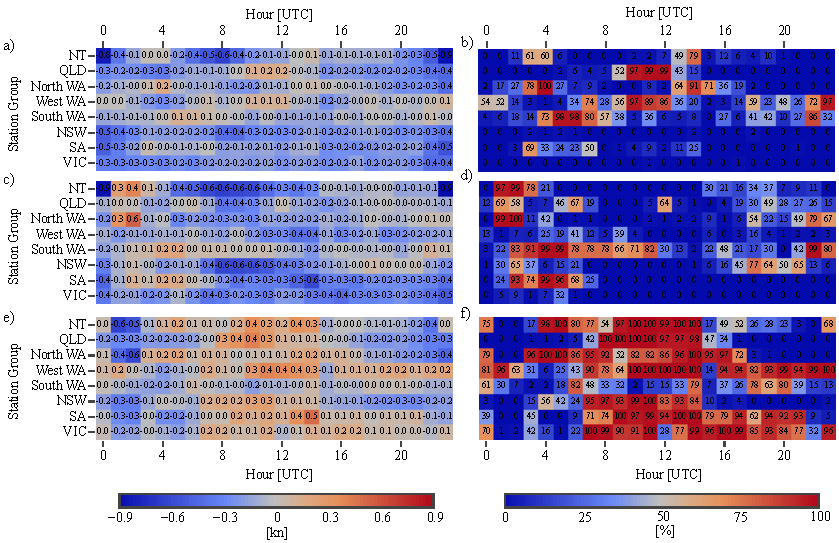
\includegraphics[width=39pc]{wpi_coastal.pdf}
\caption{Heatmaps of $\overline{\text{WPI}}$ values and confidence scores for each coastal station group and hour of the day: a) and b), Official versus ACCESS, c) and d) Official versus ECMWF, e) and f) ECMWF versus ACCESS. Positive $\overline{\text{WPI}}$ values mean that the former dataset in each pair is on average closer to observations than the latter dataset. Confidence scores provide the probability the population $\overline{\text{WPI}}$ is greater than zero. Values within the heatmaps are accurate to two significant figures.}
\label{Fig:wpi_coastal}
\end{figure*}

\begin{figure}
\centering
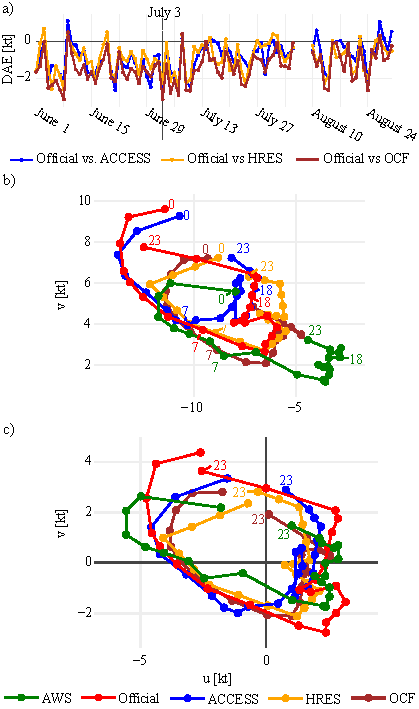
\includegraphics[width=19pc]{case_studies_nt.pdf}
\caption{Time series, a) and b), of $\overline{\text{WPI}}_\text{OA}$ and $\overline{\text{WPI}}_\text{OE}$ for, a), the NT station group at 23:00 UTC, and b), the south WA station group at 05:00 UTC. Hodographs, c) to f), showing change in winds, c) and e), and wind perturbations, d) and f), for the NT station group, c) and d), and south WA station group, e) and f).}
\label{Fig:case_studies_nt}
\end{figure}

Figures \ref{Fig:case_studies_nt} and \ref{Fig:case_studies_wa} provide case studies of the NT and South WA station groups, respectively. Figure \ref{Fig:case_studies_nt} a) provides a time series of WPI for the NT station group at 23:00 UTC. The time series shows significant temporal variability, with WPI frequently exceeding $-2$ kn. \textcolor{red}{The time series in Figures \ref{Fig:case_studies_nt} and \ref{Fig:case_studies_wa} are perhaps unnecessary, but I included them because they show both variability, and the lack of temporal autocorrelation in WPI.} Figures \ref{Fig:case_studies_nt} b) and c) show hodographs of the winds and wind perturbations, respectively, for the AWS observations, Official forecast, and ACCESS and ECMWF model datasets, at each hour UTC on the 3\textsuperscript{rd} of July, which provides an interesting example. 

Figure \ref{Fig:case_studies_nt} b) shows that the Official wind forecast on this day was likely based on edited ACCESS from 00:00 to 06:00 UTC, then edited ECMWF from 07:00 to 13:00 UTC, then unedited ACCESS from 15:00 to 21:00 UTC. The final two hours of the forecast show the Official winds acquiring a stronger east-northeasterly component than either the AWS observations, ACCESS, or ECMWF. This rapid change is clearer in the perturbation hodograph shown in Fig.~\ref{Fig:case_studies_nt} c). At this time of year the prevailing winds throughout the NT are east-southeasterly, and 22:00 UTC corresponds to $\approx$ 08:30 local solar time (LST) in this region, so the rapid departure of the Official forecast from ACCESS at this time likely represents an edit made by a forecaster to capture boundary layer mixing processes. Figure \ref{Fig:perth_sounding} a) shows the first ten values from wind soundings at Darwin Airport at 12:00 UTC on July 3\textsuperscript{rd} and 00:00 UTC on July 4\textsuperscript{th}. In both instances the winds are indeed east-southeasterly, and so the rapidly changing wind perturbations at 22:00 UTC in the Official forecast likely reflect a boundary layer mixing edit that has been applied either too early, or has strengthened the southeasterly component of the winds too much. Similar issues create low WPI scores on the 8\textsuperscript{th} of June and 9\textsuperscript{th} and 10\textsuperscript{th} of July.

Figure \ref{Fig:case_studies_wa} a) provides a time series of WPI for the South WA station group at 05:00 UTC. As with the NT station group there is significant temporal variability, with WPI frequently exceeding 1 kn. Figures \ref{Fig:case_studies_wa} b) and c) provides hodographs of the winds and wind perturbations, respectively, on the 9\textsuperscript{th} of June, which is an interesting example. The perturbation hodograph shows both ECMWF and ACCESS underpredicting the amplitude of the diurnal wind cycle on this day. In each dataset the 05:00 UTC perturbations are westerly to northwesterly, and given the orientation of the South WA coastline (see Fig.~\ref{Fig:map}) and the fact that 05:00 UTC corresponds to $\approx$ 13:00 local solar time (LST) in this region, the perturbations likely indicate boundary layer mixing processes. 

\begin{figure}
\centering
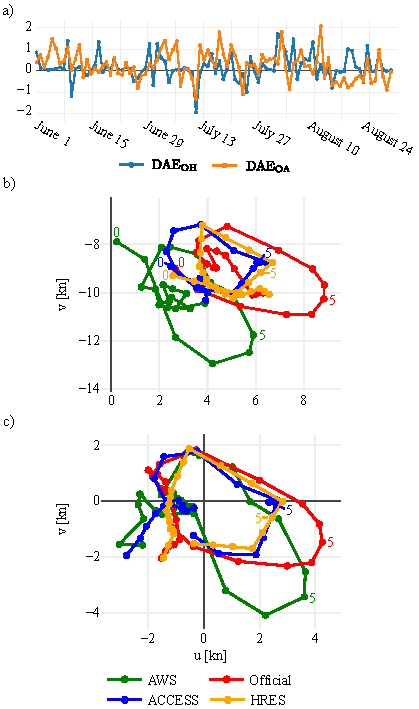
\includegraphics[width=19pc]{case_studies_wa.pdf}
\caption{Time series, a) and b), of $\overline{\text{WPI}}_\text{OA}$ and $\overline{\text{WPI}}_\text{OE}$ for, a), the NT station group at 23:00 UTC, and b), the south WA station group at 05:00 UTC. Hodographs, c) to f), showing change in winds, c) and e), and wind perturbations, d) and f), for the NT station group, c) and d), and south WA station group, e) and f).}
\label{Fig:case_studies_wa}
\end{figure}

\begin{figure*}
\centering
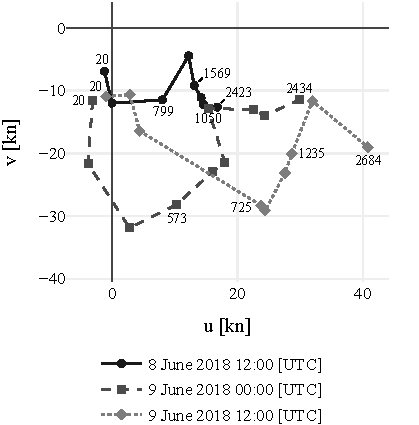
\includegraphics[width=33pc]{perth_sounding.pdf}
\caption{Hodographs showing change in winds with height at, a), Darwin Airport, and b), Perth Airport.}
\label{Fig:perth_sounding}
\end{figure*}

Figure \ref{Fig:perth_sounding} shows wind sounds throughout the first two km of the atmosphere between 12:00 UTC on the 8\textsuperscript{th} June and 12:00 UTC on the 9\textsuperscript{th} June; the soundings were taken at Perth Airport, which is the nearest station to the South WA station group to provide wind soundings. The 8\textsuperscript{th} June 12:00 UTC sounding shows surface northerlies of $\approx 6$ kn, becoming west to northwesterlies of over 20 kn $2.4$ km above the surface. A forecaster basing a model edit of the following days winds on this sounding would therefore gradually strengthen the westerly component of the surface winds in the hours after sunrise. However, the subsequent sounding at 00:00 UTC on the 9\textsuperscript{th} of June shows that the winds acquire a strong northerly component of 30 kn in the first 500 m of the atmosphere, with the final sounding indicating a strong northwesterly wind at 725 m persisting until 12:00 UTC. In Fig.~\ref{Fig:case_studies_wa} c), the Official perturbations from 04:00 to 07:00 UTC show stronger westerly perturbations than either ACCESS or ECMWF, improving the amplitude of Official's diurnal wind cycle. However, the AWS perturbations are more northerly than those of Official, and so the Official forecast winds have been strengthened in a slightly incorrect direction. One explanation for this discrepancy is that the Official forecast has been edited based on the June 8\textsuperscript{th} 12:00 UTC sounding, with the winds above the surface changing direction in the subsequent 12 hours. A similar explanation can be given for the high WPI scores on the  3\textsuperscript{rd} of August, although in this case the Official forecast slightly improves both the magnitude and direction of the 05:00 UTC wind perturbations.

\begin{figure*}
\centering
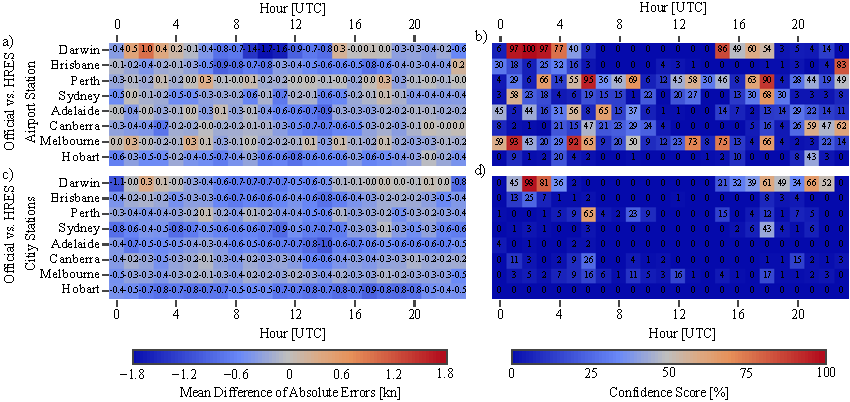
\includegraphics[width=39pc]{airport_wpi.pdf}
\caption{The $\overline{\text{WPI}}_\text{OE}$ (Official versus ECMWF comparison) values, a) and c), and confidence scores, b) and d), for the airport stations, a) and b), and airport station groups, c) and d), respectively.}
\label{Fig:airport_wpi}
\end{figure*}

To provide a contrast to the coastal station group results, Fig.~\ref{Fig:airport_wpi} presents the $\overline{\text{WPI}}$ values and confidence scores for $\overline{\text{WPI}}_\text{OE}$, which represents the Official versus ECMWF comparison, for the airport stations, and airport station groups. The results for the airport stations are noisier than the results for the coastal station groups in Figs.~\ref{Fig:wpi_coastal} c) and d), although they share some similarities. Official outperforms ECMWF at 01:00 and 02:00 UTC at both the Darwin airport station and the NT station group, although ECMWF outperforms Official between 08:00 and 14:00 UTC at Darwin and Brisbane airports, and the corresponding NT and QLD station groups, with the exception of the QLD station group at 12:00 UTC. ECMWF also outperforms Official at Hobart airport at almost all hours of the day, and at Adelaide and Canberra airports from 11:00 to 14:00 UTC. 

For the remaining stations and times, Official only outperforms ECMWF at the Perth airport station at 06:00 UTC and the Melbourne airport station at 01:00 UTC, although in both cases WPI values are comparatively small in magnitude. Furthermore, in both cases there is no clear pattern to the $\overline{\text{WPI}}_\text{OE}$ values over the rest of the day. Note that the \textit{multiplicity problem} \citep[p. 178]{wilks11} requires care be taken before giving meaning to these two examples: i.e., given that we are calculating twenty four confidence scores for eight stations, then if WPI were uncorrelated across each station and hour we would expect to find $0.05 \times 24 \times 8 \approx 10$ instances where $P\left(W_{OE}>0\right)\geq 95\%$, even if $W_{OE}$ were in fact equal to zero.

For the airport station groups, ECMWF outperforms Official for the majority of station groups and times. The main exception is the Darwin airport station group, where Official outperforms ECMWF at 02:00 UTC, ambiguity as to whether Official or ECMWF performs better at 01:00, 03:00 and 04:00 UTC, and from 15:00 to 22:00 UTC. In the analogous $\overline{\text{WPI}}_\text{OA}$ Official versus ACCESS comparisons (not shown), the airport station results are similarly noisy, although the airport station group results are slightly more favourable to Official, with Official outperforming ACCESS from 10:00 to 12:00 UTC at the Brisbane station group, and fewer occasions overall where ACCESS outperforms Official than ECMWF does. 

\begin{figure*}
\centering
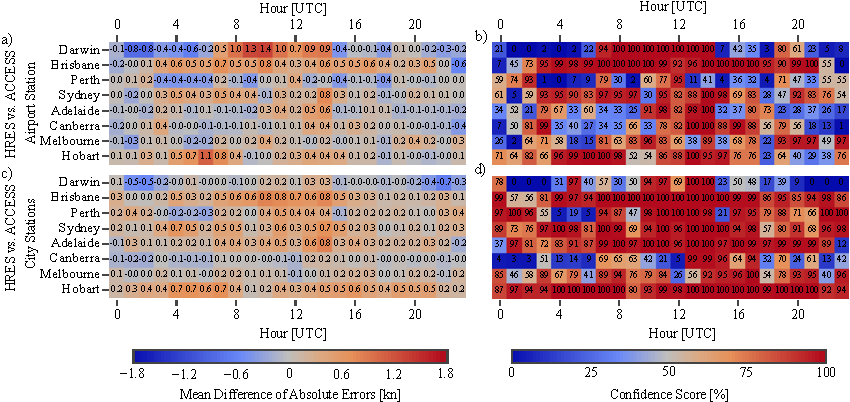
\includegraphics[width=39pc]{airport_wpi_EA.pdf}
\caption{As in Fig.~\ref{Fig:airport_wpi}, but for the $\overline{\text{WPI}}_\text{EA}$ (ECMWF versus ACCESS comparison) values and confidence scores.}
\label{Fig:airport_wpi_EA}
\end{figure*}

Figure \ref{Fig:airport_wpi_EA} presents the $\overline{\text{WPI}}$ values and confidence scores for $\overline{\text{WPI}}_\text{EA}$, which represents the ECMWF versus ACCESS comparison, for the airport stations, and airport station groups. As with the Official versus ECMWF comparison in Fig.~\ref{Fig:airport_wpi}, the results for the airport stations are noisy, but more often than not show that ECMWF outperforms ACCESS. The results for the airport station group show ECMWF usually outperforms ACCESS, the main exceptions being the Darwin and Canberra airport station groups. \textcolor{red}{Might be interesting to note that ACCESS-C+ does not run over Darwin or Canberra, possibly explaining the better performance of ACCESS there.}

Naively, the fact that ECMWF generally outperforms ACCESS at these scales is surprising, as ACCESS runs at a higher spatiotemporal resolution than ECMWF, and is calibrated for Australian conditions. However, these results are not surprising in light of the mesoscale verification challenges discussed in section \ref{Sec:Introduction}. The AWS data resolves motion with time scales as low as 10 minutes, and at arbitrarily small spatial scales: it therefore includes more unpredictable turbulence than either model dataset. Furthermore, because ACCESS runs at higher spatiotemporal resolutions than ECMWF, it includes additional scales of motion, and therefore adds additional variability to the wind fields. Unless the additional variability in ACCESS is perfectly correlated with observations, the average of $\left\lvert \boldsymbol{u}_{\text{AWS}}-\boldsymbol{u}_{\text{A}} \right\rvert$
will therefore increase, unless this additional variability is compensated for by a reduction in bias, i.e.$\left\lvert \overline{\boldsymbol{u}}_{\text{AWS}}-\overline{\boldsymbol{u}}_{\text{A}} \right\rvert$ decreases. These ideas are discussed in greater detail in section \ref{Sec:Discussion}. Note finally that the results for the Official versus ECMWF comparison in Fig.~\ref{Fig:airport_wpi} largely mirror those of the ECMWF versus ACCESS comparison in Fig.~\ref{Fig:airport_wpi_EA}, suggesting that similar arguments apply to Official, as it as based on both ACCESS, ECMWF as well as forecaster edits, which contribute additional variability.  

\subsection{Seasonal Comparison}
\label{Sec:Seasonal}
Figure \ref{Fig:cwpi_coastal} provides the Climatological Wind Perturbation Index (CWPI) values and confidence scores for the coastal station groups for $\text{CWPI}_\text{OA}$, $\text{CWPI}_\text{OE}$ and $\text{CWPI}_\text{EA}$, which represent the the Official versus ACCESS, Official versus ECMWF, and ECMWF versus ACCESS comparisons, respectively. At the NT station group Official outperforms both ACCESS and ECMWF at 03:00 UTC with reasonably confidence. However, both ACCESS and ECMWF outperform Official at 23:00 and 00:00 UTC, consistent with the $\overline{\text{WPI}}$ results of Fig.~\ref{Fig:wpi_coastal}. The NT station group results are discussed in more detail in section \ref{Sec:Discussion}.

At the North WA station group at 01:00, 03:00 and 04:00, Official outperforms ACCESS with confidence scores of 77, 78 and 90\%, respectively; Official also outperforms ECMWF at 01:00 and 02:00 UTC with confidence scores above 99\%. Figure \ref{Fig:clim_hodo} a) shows that ECMWF's poor performance at 01:00 and 02:00 UTC is simply due to its linear interpolation at these times, whereas Official's very slight outperformance of ACCESS at 01:00, 03:00 and 04:00 is due to ACCESS's climatological diurnal cycle being slightly out of phase with that of the AWS observations, and the Official forecast correcting for this somewhat. Both Official and ECMWF slightly exaggerate the magnitude of the climatological sea-breeze, which peaks around 09:00 UTC, with ACCESS performing well in this respect.

At the South WA station group from 01:00 to 05:00 UTC, Official outperforms ECMWF with confidence scores of at least $88\%$. Figure \ref{Fig:clim_hodo} b) shows that ECMWF underestimates the westerly perturbations at these times, with these perturbations likely associated with boundary layer mixing processes, as discussed in section \ref{Sec:Daily}. Each of Official, ACCESS and ECMWF noticeably underestimate the amplitude of the diurnal cycle between 02:00 and 10:00 UTC, including both the westerly perturbations and the southerly sea-breeze perturbations. 

At the NSW station group from 17:00 to 19:00 UTC, Official outperforms both ACCESS and ECMWF with confidence scores of at least least 95\% and 75\%, respectively. Figure \ref{Fig:clim_hodo} c) shows that these times correspond to ``dimples" in the perturbation hodographs that are present in all four datasets. The Official hodograph closely resembles that of ACCESS, except for this dimple, which has been exaggerated relative to ACCESS. \textcolor{red}{Don't know what is going on here.} Figure \ref{Fig:clim_hodo} c) also shows that although ECMWF exaggerates the amplitude of the easterly sea-breeze perturbations, it captures the narrower shape of the AWS hodograph better than Official or ACCESS.

At the SA station group from 02:00 to 05:00 UTC and 09:00 to 12:00 UTC, Official outperforms both ACCESS and ECMWF, although confidence scores do not exceed 88\% and 65\% respectively. Figure \ref{Fig:clim_hodo} d) shows that although the Official forecast captures the amplitude of the perturbations from 01:00 to 05:00 UTC almost perfectly, its diurnal cycle is out of phase with that of the AWS during this period, explaining why Official only slightly outperforms ACCESS in the results of Figures \ref{Fig:cwpi_coastal} a) and b).

\begin{figure*}
\centering
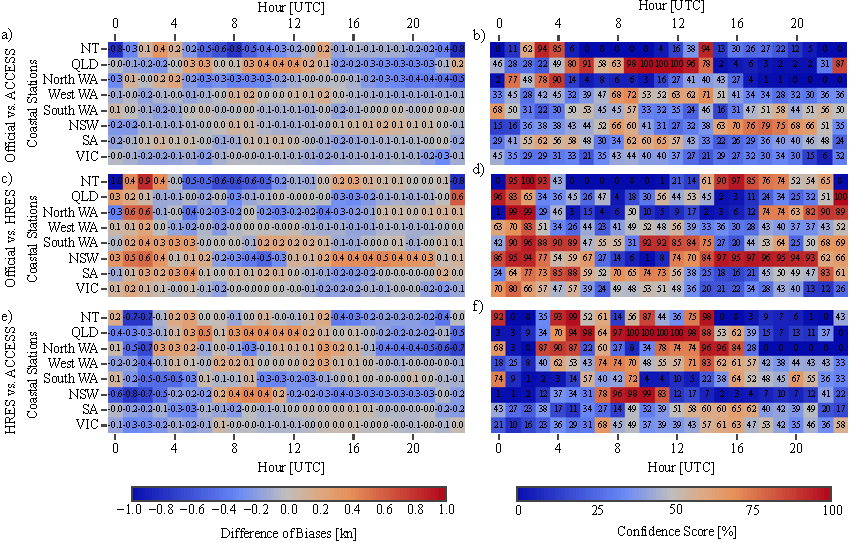
\includegraphics[width=39pc]{cwpi_coastal.pdf}
\caption{As in Fig.~\ref{Fig:wpi_coastal}, but for the CWPI values and confidence scores.}
\label{Fig:cwpi_coastal}
\end{figure*}

\begin{figure*}
\centering
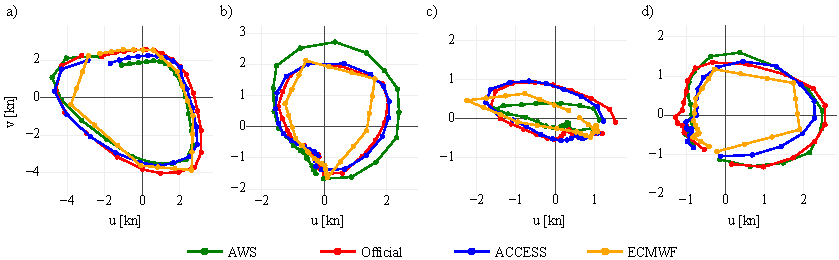
\includegraphics[width=33pc]{clim_hodo.pdf}
\caption{Climatological hodographs.}
\label{Fig:clim_hodo}
\end{figure*}

\begin{figure*}
\centering
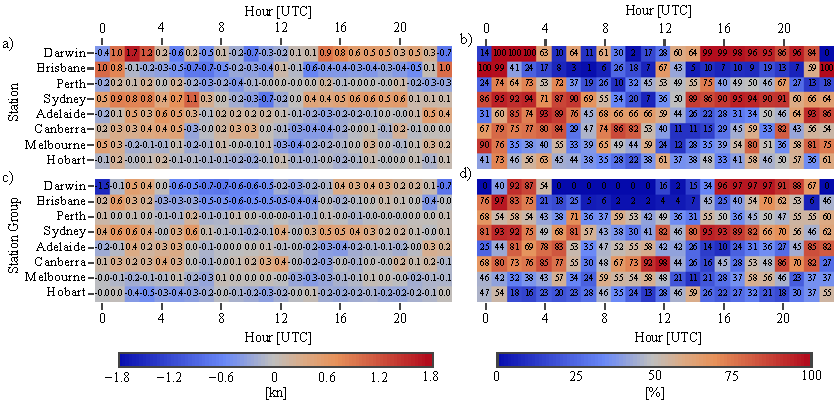
\includegraphics[width=39pc]{airport_cwpi.pdf}
\caption{As in Fig.~\ref{Fig:airport_wpi}, but for the cwpi values and confidence scores.}
\label{Fig:airport_cwpi}
\end{figure*}

For constrast, Fig.~\ref{Fig:airport_cwpi} presents the CWPI values and confidence scores for $\text{CWPI}_\text{OE}$, which represents the Official versus ECMWF comparison, for the airport stations, and airport station groups. These results show much greater similarity with the Official versus ECMWF comparisons at the coastal station groups shown in Figs.~\ref{Fig:cwpi_coastal} c) and d), than do the analogous $\overline{\text{WPI}}$ results in Fig.~\ref{Fig:airport_wpi} and Figs.~\ref{Fig:wpi_coastal} c) and d). This likely because the temporal averaging has reduced the additional unpredictable variability in Official, revealing biases in Official and ECMWF that are partly shared across the three spatial scales. This point is discussed further in section \ref{Sec:Discussion}. 

\begin{figure}
\centering
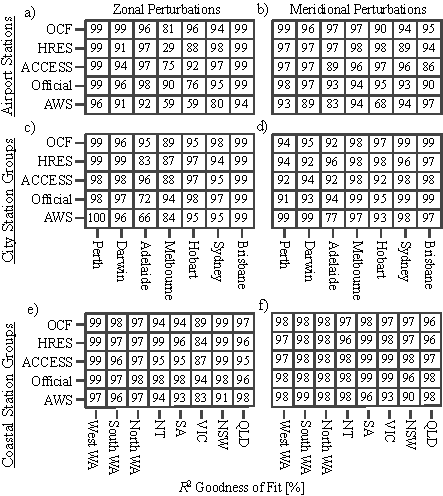
\includegraphics[width=19pc]{r_squared.pdf}
\caption{\textcolor{red}{Could also provide an analogous figure showing the use of the function $\alpha$ provides a significant improvement over the basic ellipse fit - or instead just quote some numbers? Or maybe these figures are entirely unnecessary?}}
\label{Fig:r_squared}
\end{figure}

Note that the hodographs in Fig.~\ref{Fig:clim_hodo} are roughly elliptical in shape, suggesting that descriptive quantities can be estimated by fitting equations (\ref{Eq:u}) and (\ref{Eq:v}) to the zonal and meridional climatological perturbations, then calculating these quantities from the fit, as described in section \ref{Sec:Methods}. Figure \ref{Fig:r_squared} provides the $R^2$ values for the fits of the zonal and meridional perturbations to equations (\ref{Eq:u}) and (\ref{Eq:v}), respectively. The fit performs best at the coastal station group spatial scale, with $R^2$ generally above $95\%$. It also performs well at the airport station and airport station group scales, with a few exceptions, including the ACCESS and Official meridional perturbations at the Canberra airport station group, and the ECMWF zonal perturbations at Melbourne airport. 

\begin{figure*}
\centering
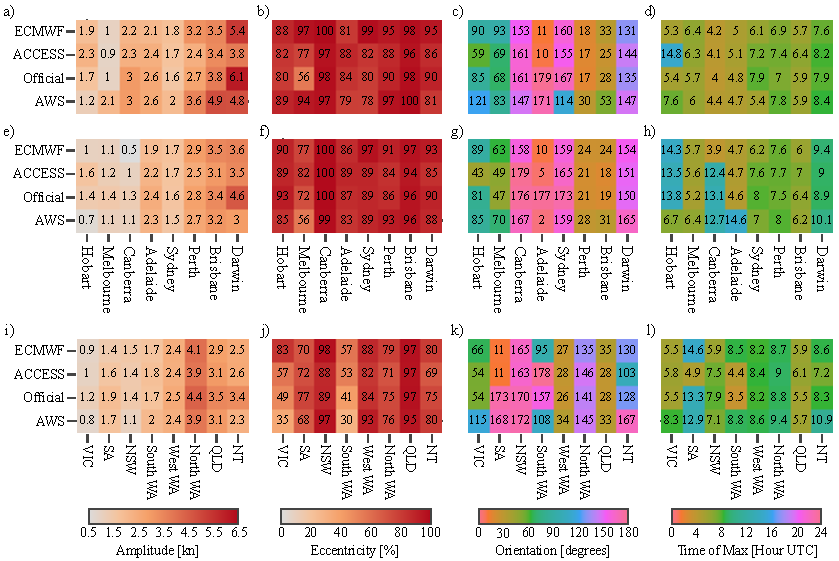
\includegraphics[width=39pc]{ellipse_fits.pdf}
\caption{Ellipse fits. \textcolor{red}{If we were to include any analysis for alternative time periods (e.g. summer 2017/18 for contrast; or could do 18/19 if I were to go back to BoM to get the data) a copy of this figure could be a good choice. Could explain changes in diurnal cycle properties, e.g. amplitude, with seasonal changes to background winds, heating, etc. Note some issues with timing and amplitude values due to asymmetry - could instead just show eccentricity and orientation values?}}
\label{Fig:ellipse_fits}
\end{figure*}

The ellipse fits are used to derive four descriptive quantities: the maximum perturbation speed, the eccentricity of the fitted ellipse, the angle the fitted ellipse's semi-major axis makes with lines of latitude, and the time maximum perturbation speed occurs. Figure \ref{Fig:ellipse_fits} provides these four quantities for each dataset and location across the three spatial scales. A variety of structural differences are apparent at a number of locations and scales. For example, Fig.~\ref{Fig:ellipse_fits} a) shows that at Brisbane airport, the maximum AWS perturbation is at least $1$ kn greater than Official, ACCESS and ECMWF, and Fig.~\ref{Fig:ellipse_fits} c) shows that the orientation of the AWS fitted ellipse is at least 20 degrees anti-clockwise from the other datasets. Figures \ref{Fig:ellipse_hodo} a) and b) show hodographs of the Brisbane airport perturbation climatology and ellipse fit, respectively. Although the ellipse fits suppress some of the asymmetric details, they capture the amplitudes and orientations of the real climatological diurnal cycles well. In this case the results show that the average AWS sea-breeze approaches from the northeast, whereas the forecast and model sea-breezes approach more from the east-northeast. To check whether this just represents a direction bias of the Brisbane Airport station, Fig.~\ref{Fig:ellipse_fits} shows the climatological perturbations at the nearby Spitfire Channel station (see Fig.~\ref{Fig:map} for the location of this station, and other stations referred to in this section). While the amplitude bias is smaller at Spitfire Channel than Brisbane Airport, the directional bias is at least as high. A similar directional bias is evident at the nearby Inner Beacon station (not shown), although the bias is smaller than at Spitfire Channel and Brisbane Airport. Thus, the directional bias in Official, ACCESS and ECMWF at these stations is likely genuine, and not just a consequence of biased AWS observations. Figure \ref{Fig:map} shows there are two small islands to the east of Brisbane airport; the more northwesterly orientation of the Brisbane Airport sea-breeze suggests these islands may be redirecting winds between the east coast of Brisbane and the west coasts of these islands, and that this local effect is not being captured in Official, ACCESS or ECMWF.            

\begin{figure*}
\centering
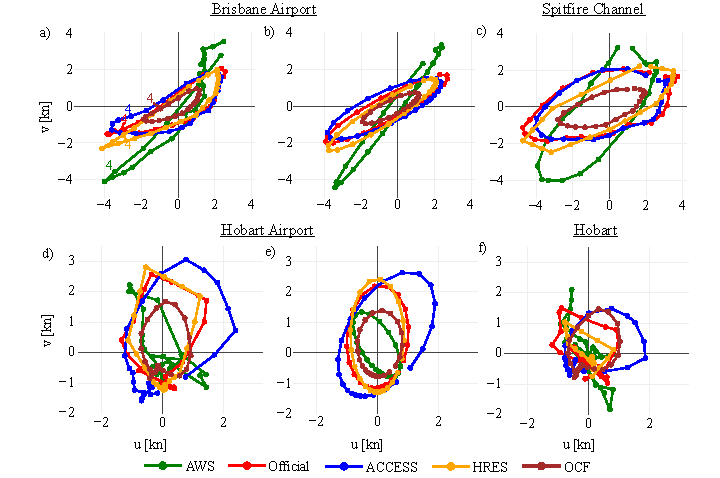
\includegraphics[width=39pc]{ellipse_hodo.pdf}
\caption{Ellipse fits. Could instead just provide one example.}
\label{Fig:ellipse_hodo}
\end{figure*}

Another example is the Hobart Airport station. Figure \ref{Fig:ellipse_fits} c) shows that the ellipse fits for the AWS perturbations are oriented 31, 35 and 62 degrees anti-clockwise from the ECMWF, Official and ACCESS ellipse fits, respectively. Figures \ref{Fig:r_squared} a) and b) show that the ellipse fit for the AWS perturbations at Hobart airport only achieve $R^2$ values of 59\% and 68\% for the $u$ and $v$ components, respectively. However, figures \ref{Fig:ellipse_hodo} d) and e) show that the fit still captures orientations accurately, although it underestimates the maximum AWS perturbation. Figure \ref{Fig:ellipse_hodo} f) shows the climatological perturbations at the Hobart (city) station, which also show a large difference in orientation between ACCESS and AWS. Given the timing of the westerly perturbations in ACCESS, and the fact that the prevailing winds around Tasmania are westerly, these results suggest that ACCESS is exaggerating the boundary layer mixing processes involved in the diurnal cycle around Hobart.

The South WA station group also provides an interesting example. Here the ACCESS and Official ellipse fits are oriented at least 49 degrees anti-clockwise from those of AWS and ECMWF, and the ECMWF perturbations peak between 1.2 and 2.5 hours after the other datasets. These differences occur because eccentricity values are low for this station group, and Figure \ref{Fig:clim_hodo} b) shows that the westerly perturbations associated with boundary layer mixing are weaker for ECMWF that the other datasets. A similar issue affects the VIC station group, explaining why the AWS ellipse fit is oriented at least 49 degrees anti-clockwise from those of the other datasets.  

The Darwin Airport, Darwin Airport station group, and NT station group provide further examples. In these cases there are timing differences between the perturbation maximums of up to 8.2 hours. Figure \ref{Fig:nt_ellipse_hodo} shows that these differences occur because for some datasets, the later north to northwesterly sea-breeze perturbations dominate the diurnal wind cycle, but for other datasets the earlier easterly to southeasterly boundary layer mixing effects dominate. 

\begin{figure*}
\centering
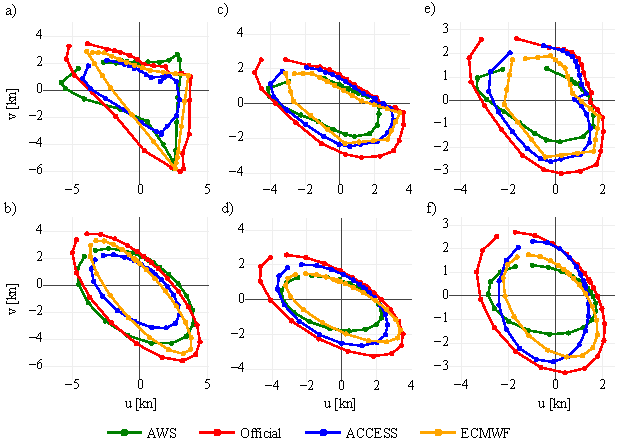
\includegraphics[width=39pc]{nt_ellipse_hodo.pdf}
\caption{Ellipse fits. \textcolor{red}{Could also include the ellipses, but this makes the figure very large.}}
\label{Fig:nt_ellipse_hodo}
\end{figure*}

\section{Discussion}
\label{Sec:Discussion}
The results of section \ref{Sec:Results} may have some confronting implications for forecasting practice. If the goal of land-sea breeze and boundary layer mixing edits is to reduce absolute errors in the following day's forecast of the surface wind fields, then a necessary (but not sufficient) condition for this to occur is for these edits to at least reduce the absolute errors in the diurnal component of the surface wind fields. However, the WPI comparisons in Figs.~\ref{Fig:wpi_coastal} and \ref{Fig:airport_wpi} suggest that this is only possible when absolute error is calculated at coarse spatial scales. If the Official forecast is based, at least partly, on an edited high resolution model guidance dataset like ACCESS, then due to the mesoscale verification issues discussed in section \ref{Sec:Introduction}, the larger absolute errors associated with a higher resolution model completely mask the effect of the edits, with a lower resolution unedited model like ECMWF scoring better overall. While the CWPI results in Figs.~\ref{Fig:cwpi_coastal} and \ref{Fig:airport_wpi} suggest that forecaster edits can improve the accuracy of diurnal wind cycles in a climatological sense, it is not clear if these improvements have operational significance. 

To investigate these ideas further, consider first just the zonal components of the AWS and Official wind perturbations, denoted by $u_\text{AWS}$ and $u_\text{O}$ respectively. Considering just the values at a particular hour UTC, at a particular station, over the entire June, July, August time period, the mean square error  $\mse\left(u_\text{AWS}, u_\text{O}\right) = \overline{\left(u_\text{AWS} - u_\text{O}\right)^2}$ can be decomposed
\begin{equation}
\mse\left(u_\text{AWS}, u_\text{O}\right) = \underbrace{\var\left(u_\text{AWS}\right) + \var\left(u_\text{O}\right) - 2 \cdot \covar\left(u_\text{AWS}, u_\text{O}\right)}_{\var\left(u_\text{AWS} - u_\text{O}\right)} + \underbrace{\left(\overline{u}_\text{AWS} - \overline{u}_\text{O}\right)^2}_{\text{squared bias}} \label{Eq:MSE}
\end{equation}
where $\var$, $\covar$ and over-bars denote the sample variance, covariance and mean respectively. The first three terms are the total variance of $u_\text{AWS} - u_\text{O}$, whereas the last term is the square of the bias between $u_\text{AWS}$ and $u_\text{O}$. Note that the mean square error $\mse\left(u_\text{AWS}, u_\text{O}\right)$ is closely related to $\overline{\text{WPI}}$, which is the difference between the mean absolute error of Official and AWS, and a model guidance dataset and AWS. Similarly, the CWPI is closely related to the squared bias component $\left(\overline{u}_\text{AWS} - \overline{u}_\text{O}\right)^2$ of the mean square error. Equation (\ref{Eq:MSE}) can also be applied to wind perturbations that have first been spatially averaged over a station group, and to $\mse\left(u_\text{AWS}, u_\text{E}\right)$ and $\mse\left(u_\text{AWS}, u_\text{A}\right)$, where $u_\text{E}$ and $u_\text{A}$ are the ECMWF and ACCESS zonal perturbations, respectively. 

\begin{figure*}
\centering
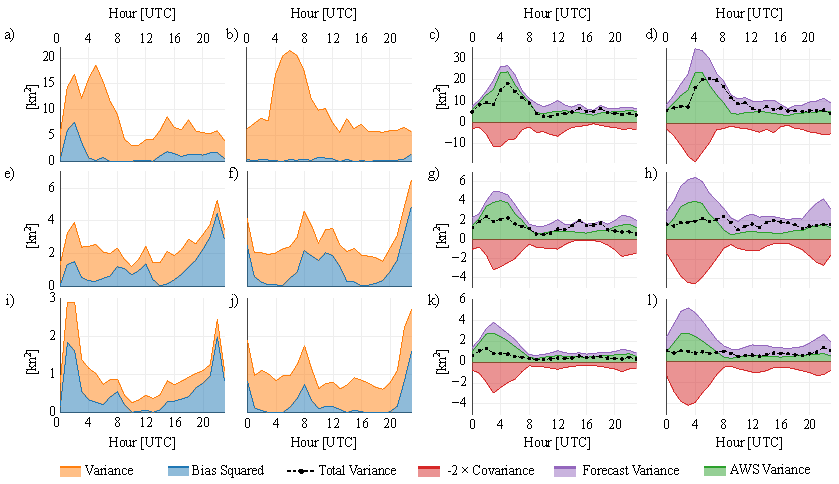
\includegraphics[width=39pc]{error_decomp.pdf}
\caption{Actual perturbation standard deviation values. Note that official performs the worst at this scale!}
\label{Fig:error_decomp}
\end{figure*}

Figure \ref{Fig:error_decomp} shows each term in the mean square error decomposition of equation \ref{Eq:MSE} for both $\mse\left(u_\text{AWS}, u_\text{O}\right)$ and $\mse\left(u_\text{AWS}, u_\text{E}\right)$, for Darwin Airport, the Darwin station group, and the NT station group. This region provides an interesting case study because Fig.~\ref{Fig:airport_wpi} shows that Official has some skill at both Darwin Airport and over Darwin Airport station groups, in contrast to most other locations. At Darwin Airport, $\mse\left(u_\text{AWS}, u_\text{O}\right)$ exceeds $\mse\left(u_\text{AWS}, u_\text{E}\right)$ from 04:00 to 16:00 UTC due to higher total variance, whereas outside of these times $\mse\left(u_\text{AWS}, u_\text{E}\right)$ exceeds $\mse\left(u_\text{AWS}, u_\text{O}\right)$ due to larger bias. The higher total variance of $u_\text{AWS} - u_\text{O}$ occurs because $\var\left(u_\text{O}\right) > \var\left(u_\text{E}\right)$. This additional variability is mostly random from 04:00 to 14:00 UTC, i.e. $u_\text{O}$ is not sufficiently correlated with $u_\text{AWS}$ at these times for the additional variability of $u_\text{O}$ to produce a reduction in mean square error. Thus, while the bias between Official and AWS is lower, or about the same, as that between ECMWF and AWS, the higher random variability of Official results in higher mean square error for most of the day. Figure \ref{Fig:error_decomp_v} shows similar conclusions can be drawn for the meridional perturbations at Darwin Airport, although in this case $\var\left(u_\text{O}\right) > \var\left(u_\text{E}\right)$ for the entire day. Most of the difference between the WPI and CWPI scores for the Official versus ECMWF comparison at Darwin Airport in Figures \ref{Fig:airport_wpi} and \ref{Fig:airport_cwpi}, respectively, can be explained through the different mean square error and bias terms for the zonal perturbations alone. 

Figure \ref{Fig:nt_ellipse_hodo} a) shows that ECMWF's climatological perturbations at Darwin Airport underestimate the easterly perturbations from 00:00 to 03:00 UTC, which are presumably associated with boundary layer mixing processes. Official does a better job of resolving these easterly perturbations, but is generally outperformed by ECMWF in resolving the northerly sea-breeze perturbations. Similar points can be made for the Darwin and NT coastal station groups. While spatial averaging reduces a portion of the unpredictable variability in Official, Official also often has larger meridional biases at these scales compared to ECMWF. Figures \ref{Fig:nt_ellipse_hodo} and \ref{Fig:ellipse_fits} show that these biases can be explained in terms of amplitude and orientation differences between Official, ECMWF and AWS. Figures analogous to Figs. \ref{Fig:error_decomp} and \ref{Fig:error_decomp_v}, but for other locations around Australia, show similar results, but without the large meridional biases present in the Official forecast at the Darwin Airport station group and NT coastal station group.   

These examples illustrate the idea that the additional unpredictable variability introduced by a higher resolution edited forecast needs to be ``paid for" by a reduction in bias, otherwise the net result will just be an increase in error. However, although a high resolution edited forecast may have higher mean squared error compared with observations than an unedited low resolution model, the former may capture variability more realistically, and hence better represent the possibility of extremes, even if the timing of these extremes is unpredictable; which of the two constitutes a better forecast therefore depends entirely on the application. For instance, in engineering applications, the possibility of wind extremes of a certain magnitude may be most important, regardless of when they occur, whereas in aviation or sailing it may be more important to minimise the mean square error. The fact that high and low resolution model guidance products are used at different times, and on different days, implies that the Official forecast is inconsistent in which measures of accuracy it intends to maximise, and more thought therefore needs to be given to this issue.  

\begin{figure*}
\centering
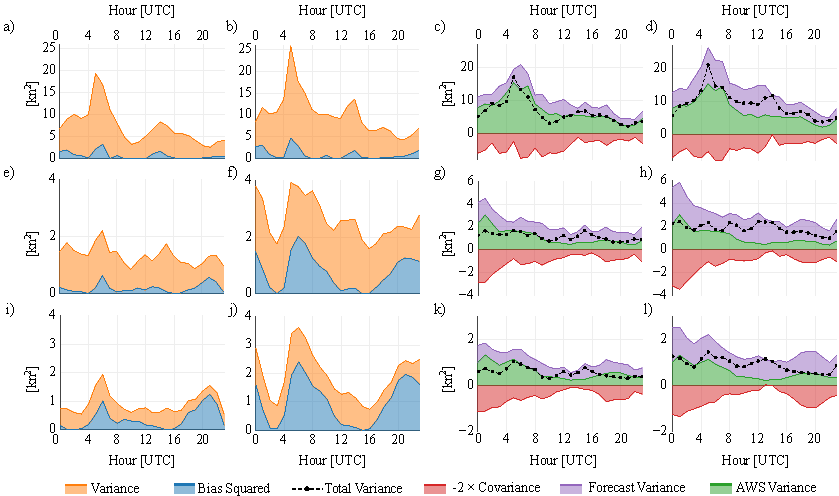
\includegraphics[width=39pc]{error_decomp_v.pdf}
\caption{Actual perturbation standard deviation values. Note that official performs the worst at this scale!}
\label{Fig:error_decomp_v}
\end{figure*}

\section{Conclusion}
\label{Sec:Conclusion}
We have

\bibliographystyle{ametsoc2014}
\bibliography{./references.bib}

\end{document}
